\section{Scaling Laws}\label{sec:scaling_laws}

% It has been known that transformer model performance has a power-law relationship with the factors: model size (N), dataset size (D) \cite{kaplan2020scaling, hoffmann2022training}. In this section, we factorize granularity as the new dimension and show how it also follows the scaling law.

Granularity determines changes in the architecture of MoE. In this section, we answer a central question of this work: whether the granular MoE models follow scaling laws and, if so, how granularity affects them. Thus, we aim to derive a parametric scaling law for predicting the final loss value $\mathcal{L}$ based on granularity $G$, total number of non-embedding parameters $N$, and number of training tokens $D$. 

% \begin{figure}[t]
% \centering
% \includegraphics[width=0.5\textwidth]{icml2024/figures/delta.pdf}
% \caption{
% Difference in the loss between training for 16B and 65B tokens for all model sizes and granularity values.
% % \marekc{I suggest to compress the model sizes to a human readable format} \janek{TODO: tak}
% }
% \label{fig:gran_project_no_interact}
% \end{figure}

% \begin{figure}[t]
% \centering
% \includegraphics[width=0.4\textwidth]{icml2024/figures/granularity_N_1082130432_D_31250.0.pdf}
% \caption{
% We plot the effect of $G$ on $\mathcal{L}_{N,D}(G)$ for constant $N$ and $D$. Both axes are in the log-scale. The results suggest the linear relationship between $\log(G)$ and $\log(\mathcal{L}-c)$.
% The given values are $N=64 \times 25M$, $D=16B$, $const=3.12$ .  The plots for additional values of $N$ and $D$ can be found in Appendix \ref{sec:app_add_viz}.
% % \marekc{I suggest to compress the model sizes to a human readable format} \janek{TODO: tak}
% }
% \label{fig:loss_nd_g}
% \end{figure}

% \begin{figure*}[t]
%   \centering
%   \begin{tabular}{ c @{\hspace{2pt}} c @{\hspace{10pt}} c}
%     \includegraphics[width=.3\textwidth]{icml2024/figures/granularity_N_1082130432_D_31250.0_new_ratio.pdf} &
%         \includegraphics[width=.302\textwidth]{icml2024/figures/kaplan_4.pdf} &
%             \includegraphics[width=.33\textwidth]{icml2024/figures/delta.pdf} \\
%     \small \textbf{(a)} &
%       \small \textbf{(b)} &
%         \small \textbf{(c)} &
%   \end{tabular}

%   \medskip

%   \caption{\textbf{(a)} We plot the effect of $G$ on $\mathcal{L}_{N,D}(G)$ for constant $N$ and $D$. Both axes are in the log-scale. The results suggest the linear relationship between $\log(G)$ and $\log(\mathcal{L}-c)$.
% The given values are $N=64 \times 25M$, $D=16B$, $const=3.12$ .  The plots for additional values of $N$ and $D$ can be found in Appendix \ref{sec:app_add_viz}. \textbf{(b)} The impact of varying the number of parameters $N$ on the loss for fixed granularity $G=4$. For other granularity values, see Appendix \ref{sec:app_add_viz}. \textbf{(c)} The difference in the loss between training for 16B and 65B tokens for all model sizes and granularity values. The model size is reported as the expansion rate and the number of active parameters.}
%   \label{empirical}
% \end{figure*}

We run over 100 experiments on the decoder-only Transformer architecture, with each \ff{} component replaced by a Mixture of Experts layer. Those experiments involve training models with sizes ranging from 129M to 3.7B parameters across different training durations, from 16B to 130B tokens. We consider logarithmically spaced values of granularity between 1 and 16. To constrain the search space, $E=64$ is fixed, following the recommendations of \cite{clark2022unified}.  In addition, we also run experiments with dense Transformers to compare their performance with MoE. The details of all architectures, the training procedure, and hyperparameter choices are described in detail in Appendix~\ref{app:setup}.

% \newpage
In the subsequent part of this paper, we will use the notation $E\times \nact$ to describe a MoE model with $\nact$ active parameters and expansion rate $E.$

% \begin{figure}[t]
% \centering
% \includegraphics[width=0.45\textwidth]{icml2024/figures/kaplan.pdf}
% \caption{
% Experimental results for a fixed granularity. Both axes are in log scale \ka{experiments for other granularities in appendix?}.
% % Scaling model and dataset size for a fixed granularity. We observe close to linear relationship in the log-log scale, which implies power law in both parameters. Dashed lines are fitted to each set of points separately for the purpose of illustration.
% } 
% \label{scaling_n_d}
% \end{figure} 
% \begin{table}[h]
%     \centering
%     \begin{tabular}{c|c}
%         \# Parameters & 25M, 50M, 100M \\
%         \hline
%         \# Training tokens & 25M, 50M, 100M \\ 
%         \hline
%         \# Granularity & 25M, 50M, 100M \\ 
%         \hline
%         \# Total runs & 25M, 50M, 100M \\ 
%     \end{tabular}
%     \caption{Compute optimal training hyper-parameters for MoE models. \sj{This importantly should have flops on the left.}}
%     \label{tab:compute_opt}
% \end{table}

% In this section we derive and validate scaling laws for MoE considering granularity, model size and number of training tokens. The details of the training setup, routing algorithm used, etc. are presented in \ref{sub:setup}.

%The star

% \begin{figure*}[ht!]
% \centering
% \includegraphics[width=0.8\textwidth]{icml2024/figures/gran_sep.png}
% \caption{Granular MoE models empirically obey similar power-law scaling when increasing model size, at least when hyper-parameters do not diverge too much from the optimum. Lines drawn here are just to visualize the trend, and are not generated by our scaling law, unlike other plots. \janek{check: To prawda? wydawało mi się, że ten plot tak był zrobiony} 
% \ka{labels should be bigger / more easily legible,
% also details like $10^0$ can be written only once at the top or so. saying number of tokens instead of number of steps?
% }
% }
% \label{fig:gran_linear}
% \end{figure*}


\newpage
\subsection{Power Law With Respect to Granularity} 
%To create a joint scaling laws formula for $N$, $D$ and $G$, we first need to investigate how $G$ determines loss independently for each $(N,D)$, analysing $L_{N,D}(G)$. 
We first answer the question of whether granular models follow the scaling laws. In Figure~\ref{fig:scalinglaws}(a), it can be seen that increasing granularity results in a lower loss. The returns follow approximately an exponential pattern, converging to a positive constant.   The empirical relationship given by Figure \ref{empirical}(a) suggests the following power-law dependence of loss on a varying granularity for given $N$ and $D$ and constants $g, h$ and $\gamma$ that may be dependent on them,
% As we already noted multiplicative relationship between $N$ and $G,$ we can assume the interaction
% \begin{align}
%     L_{D}(N, G) = \left(\frac{C}{G^\gamma} + c\right)\frac{1}{N^\alpha} + A.
% \end{align}
% \janek{TODO rewrite paragraphs above, using arguments from previous version and a plot. Prove that on loss/granularity plot with constant N and D we can see the following equation. I think that now it's enough to prove that this equation is correct independently for any N and D}:
\begin{align}\label{eq:g_only}
    \mathcal{L}_{N,D}(G) = \frac{g_{N,D}}{G^{\gamma_{N,D}}} + h_{N,D}.
\end{align}
%\ps{Ja nie rozumiem tej dyskusji, czy ktoś to może przepisać/rozwinać? Też $x$ jest nie wprowadzonym wcześniej oznaczeniem, więc nie jest jasne jaką rolę odgrywa.}
\begin{figure*}[t]
  \centering
  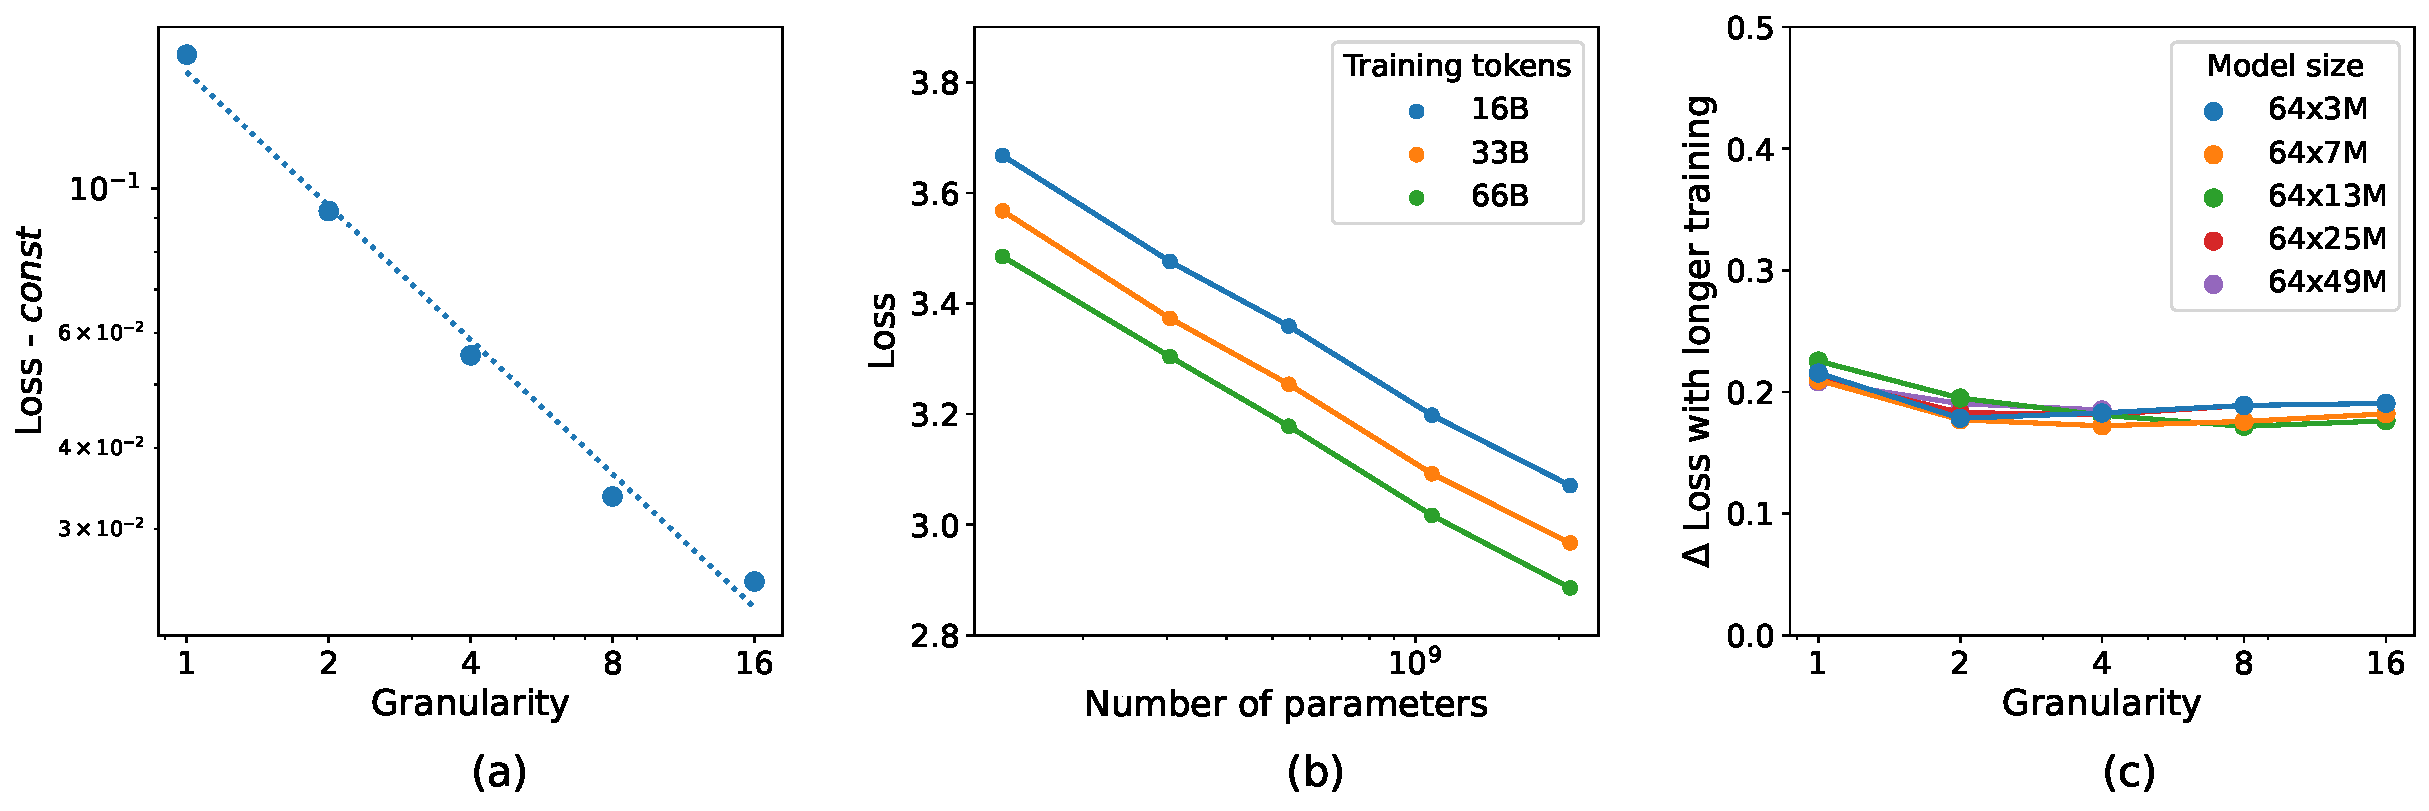
\includegraphics[width=.99\textwidth]{figures/derivation_formula.pdf}
  % \medskip
  \caption{\textbf{(a)} The effect of $G$ on $\mathcal{L}_{N,D}(G)$ for constant $N$ and $D$. Both axes are in the log-scale. The results suggest the linear relationship between $\log(G)$ and $\log(\mathcal{L}-c)$.
The given values are $N=64 \times 25M$, $D=16B$, $const=3.12$ .  The plots for additional values of $N$ and $D$ can be found in Appendix \ref{sec:app_add_viz}. \textbf{(b)} The impact of varying the number of parameters $N$ on the loss for fixed granularity $G=4$. For other granularity values, see Appendix \ref{sec:app_add_viz}. \textbf{(c)} The difference in the loss between training for 16B and 65B tokens for all model sizes and granularity values. The model size is reported as the expansion rate and the number of active parameters.}
  \label{empirical}
\end{figure*}
\subsection{Scaling the Model and Dataset Size}
\label{sec:scaling_model_data}
As outlined in Section~\ref{sec:back_scaling}, the power-law given by Eq.~\ref{eq:chinchilla} consists of three terms that describe inherent data entropy and limitations in function representation and data. This derivation is independent of the architecture. In particular, the Eq.~\ref{eq:chinchilla} also holds for constant granularity. Empirically, we observe a power law relationship in $N$ and $D$ analogous to that in dense models as depicted in Figure~\ref{empirical}(b) for a fixed value of granularity (see also Fig.~1, \cite{kaplan2020scaling}).  Furthermore, the validity of this functional form is verified by fit in Section~\ref{sub:parametric}. 

Since we know that separate scaling laws are valid for given granularities, in the general form, the parameters in Eq.~\ref{eq:chinchilla} can be dependent on the model's granularity:
\begin{align}\label{eq:gran_func}
     \mathcal{L}_G(N, D) = c_G + \frac{a_G}{N^{\alpha_G}} + \frac{b_G}{D^{\beta_G}}.
\end{align}


%In order to obtain an equation modeling the loss for a fixed granularity, we can follow the discussion presented in~\cite{hoffmann2022training}. Despite changes in the architecture in MoE models, the size of the hypothesis space depends on the number of parameters. Similarly, the stochastic approximation term is determined by the dataset size. Therefore, we expect Eq.~\ref{eq:chinchilla} to also hold in this context. 

% \jk{poprzedni tekst poniżej:}
% In our experiments, we empirically observe that the power-law given by Eq.~\ref{eq:chinchilla} also holds for granular models. Empirical observations reveal a linear relationship between the logarithm of the loss function and the logarithm of the number of non-embedding parameters, consistent across varied granularity and token counts. Fig. \ref{scaling_n_d}, on a log-scale depicts a linear relationship between the number of parameters $N$ and the loss $L$ for constant granularity. The linear relationship holds for multiple values of the number of tokens $D$ whose impact is incorporated into the constant of the linear equation. Fig~\ref{scaling_n_d} presents the analogous case where the linear relationship holds between the loss and the number of tokens.

\subsection{The Form of the Joint Scaling Law}\label{sub:joint}


%The key question of this work is how granularity $G$ can follow scaling laws.  %Below we make several observations on the restrictions on the formula and derive its final form. 
Following the above observation that models with constant granularity obey Chinchilla scaling laws given by Eq.~\ref{eq:chinchilla}, the key question arises as to how the general notion of granularity $G$ can be incorporated into the joint scaling law. %, sharing the formula across all granularities.
Moreover, the scaling law formula from Eq.~\ref{eq:gran_func} for constant $N$ and $D$ has to be representable by Eq. \ref{eq:g_only}. This is because the former is a more general equation, encompassing shared hyper-parameters across all $N$, $D$, and $G$. It is anticipated to align with the latter, consisting of distinct power laws, each with specific parameters for different $N$ and $D$ values. Consequently, the objective is to identify a function that fulfills these criteria.

%because the former is a more general equation, sharing hyper-parameters for all $N$, $D$ and $G$ and we should expect that it matches the latter, which represents set of separate power laws, with specific parameters for each $N$ and $D$ \sj{that sentence is way too long and complicated}. \jk{podoba mi się to zdanie, można je jednak podzielić} This means, that we want to find a function that satisfies: 
\begin{align}\label{eq:l_general}
% \begin{array}{lll}
     \mathcal{L}(N, D, G) &= \hspace{0.43cm} \mathcal{L}_{N,D}(G)  \hspace{0.43cm} = \hspace{0.6cm} \mathcal{L}_G(N,D) & \\
      &= \frac{g_{N,D}}{G^{\gamma_{N,D}}} + h_{N,D} = c_G + \frac{a_G}{N^{\alpha_G}} + \frac{b_G}{D^{\beta_G}} & \nonumber
% \end{array}
\end{align}
%In general form, the parameters in Eq.~\ref{eq:chinchilla} are assumed to be functions of the model's granularity:
%\begin{align}\label{eq:gran_func}
     %L_G(N, D) = C_G + \frac{A_G}{N^{\alpha_G}} + \frac{B_G}{D^{\beta_G}}.
%\end{align}
%\begin{align}\label{eq:gran_func}
 %   L(N, D, G) = L_0' + \frac{a}{N(G)^{\alpha}} + \frac{b}{D(G)^{\beta}} +G(G),
%\end{align}

% \begin{align}\label{eq:gran_func}
%     L(N, D, G) = L_0(G) + \frac{A(G)}{N^{\alpha(G)}} + \frac{B(G)}{D^{\beta(G)}}.
% \end{align}
In the subsequent sections, we aim to determine which of these parameters remain independent of $G$ and identify their functional form. Furthermore, we present some rationale for the structure of our formula.


\textbf{Lower Bound.}
Consider the limit of Eq.~\ref{eq:gran_func} for $N$ and $D$ growing to infinity:
\begin{align}\label{eq:gran_limit}
\lim_{\substack{N\to \infty\\ D\to \infty}}    \mathcal{L}(N, D, G) = c_G.
\end{align}
% As argued in Sec. \ref{sec:scaling_model_data}, the bound of the achievable loss when training bigger models on more samples should not be dependent on the architecture. Hence, 
% we get $\mathcal{L}_0(G) = L_0$, and 
% One possible solution is to include $G$ as an individual factor, with a similar role to $N$ and $D.$ This would lead to the equation
% \begin{align}\label{eq:gran_summand}
%     L(N, D, G) = L_0' + \frac{C}{G^\gamma} + \frac{A(G)}{N^{\alpha(G)}} + \frac{B(G)}{D^{\beta(G)}}.
% \end{align}
% %\marekc{Perhaps we write "with growing $N$ and $D$ the loss converges to" instead of "reduces to"?} 
% Note however that with growing $N$ and $D$ and a fixed $G$, Equation \ref{eq:gran_func} converges to
% \begin{align}\label{eq:gran_summand_const}
%     L_G(N, D) = L_0' + L_G + \frac{A'}{N^{\alpha'}} + \frac{B'}{D^{\beta'}},
% \end{align}
% \begin{align}\label{eq:gran_summand_const}
%     L_0(G) = L_0' +  \frac{C}{G^\gamma} 
% \end{align}
 with the constant term $c_G$ dependent on granularity. This is contradictory to the fact that it captures the inherent entropy of the dataset. Lower bound of the achievable loss when training bigger models on more samples should not depend on the architecture, therefore parameter $c_G=c$ is constant for all granularities. 
%the expected form of the equation can be reduced to
%\begin{align}\label{eq:}
%    L(N, D, G) = L_0 + \frac{a}{N(G)^{\alpha'}} + \frac{b}{D(G)^{\beta'}},
%\end{align}
 %\begin{align}
     %L(N, D, G) = L_0 + \frac{A(G)}{N^{\alpha(G)}} + \frac{B(G)}{D^{\beta(G)}},
 %\end{align}
%with the second and third terms capturing interactions between granularity and the size of the model and dataset respectively. In the next part of this section, we will describe these interactions based on empirical data.
% The key problem is then understanding interactions between granularity and other parameters, that is the number of tokens $D$ and the number of parameters $N$. Fig.~\ref{fig:gran_project} describes the linear relationship between the number of parameters and loss as seen also in Fig.~\ref{scaling_n_d}. However, Fig.~\ref{fig:gran_project} presents the lines for several granularity values.




\textbf{Granularity and Number of Tokens $D$.} 
As seen in Figure~\ref{empirical}(c), the benefit of training a model on a larger dataset is almost the same for each granularity value. This suggests that there is no interaction between $D$ and $G$. Therefore, we can assume that 

%\begin{align}
    %\frac{b}{D(G)^{\beta}} = %\frac{b}{D^\beta},
%\end{align}
 \begin{align}
     \frac{b_G}{D^{\beta_G}} = \frac{b}{D^\beta}.
\end{align}

%leaving us with:
% \begin{align} \label{eq:gran_no_d}
%      L(N, D, G) = c + \frac{a_G}{N^{\alpha_G}} + \frac{b}{D^\beta}.
% \end{align}

%\begin{align} \label{eq:gran_no_d}
%    L(N, D, G) = L_0 + \frac{a}{N(G)^{\alpha'}} + \frac{b}{D^\beta},
%\end{align}

%\jk{poprzednia wersja:}
%\begin{align}
%    L(D, G) = \frac{B}{D^\beta}.
%\end{align}
%Fig.~\ref{fig:gran_project_no_interact} presents three plots for different values of the number of tokens $D$. The shapes of the presented lines in each of the plots are very similar but differ in their relative position on the vertical axis. The larger steps result in lower loss values, suggesting the number of tokens can be incorporated into the constant and does not affect the loss independently from granularity. 



% \begin{figure*}[ht!]
% \centering
% \includegraphics[width=0.6\textwidth]{icml2024/figures/final_scaling.pdf}
% \caption{We present the fit of the scaling law compared to experimental results. }
% \label{fig:scalinglaws}
% \end{figure*}

% \begin{figure*}[t]
%   \centering
%   \begin{tabular}{ c @{\hspace{5pt}} c @{\hspace{100pt}}}
%     \includegraphics[width=.725\textwidth]{icml2024/figures/final_scaling.pdf} &
%       \includegraphics[width=.27\textwidth]{icml2024/figures/validation.pdf} \\
%     \small \textbf{(a)} &
%       \small \textbf{(b)}
%   \end{tabular}

%   \medskip

%   \caption{\textbf{(a)} Fit of the scaling laws compared to the experimental results. \textbf{(b)} Validation of the fit. }
%   \label{fig:scalinglaws}
% \end{figure*}



%\jk{tak naprawdę chyba najlepiej byłoby sparafrazować to zdanie ze sparse scaling laws (mamy te same wyniki): the model size power law scaling for all granularity levels differs primarily in
%a constant factor (intercept in a log-log plot); $\alpha$ stays consistent.}
%

%\janek{Brakuje tutaj jakiegoś plota uzasadniającego, że samą zmianę granularity możemy modelować power law, przy stałych tokenach i parametrach. Nie ma też argumentu, czemu nie ma granularity nie ma w wykładniku. Coś tego typu musi sie tu znaleść: Similarly to (sparse scaling) \cite{sparsescalinglaws} we let the exponents be independent of granularity, since this would either break the simple power law relationship between granularity and perplexity or introduce too much parameters and complexity for extrapolations to be reliable and parametric fitting to be numerically stable, however we think that approach this might be a promising direction for the future, but this goes beyond the scope of this work. }






% \janek{ponizej text do przepisania na argumentacje eq 10 z L(G)}

% \textbf{Granularity and model size.} 
% In Fig. \ref{fig:parallel_better}, we see that the loss values for a varied model size form almost parallel curves, characterized by granularity. Thereby, a certain change in the value of $G$ shifts the loss by the same amount for each model size. This linear relationship on the log-log scale translates into a multiplicative interaction between $N$ and $G$. 


%\begin{figure}[ht!]
%\centering
%\includegraphics[width=0.47\textwidth]{icml2024/figures/lines_shorter_2.png}
%\caption{
%Loss values for models trained on a fixed number of tokens. Dotted lines are fit separately to each set of points for the purpose of illustration.
%\sj{Steps into tokens; parameters into 20k/20M etc., round them up/down. In general those charts seem a bit random.} \janek{I jaka tu jest skala na %osi y, to jest log?} 
%}
%\label{fig:parallel_better}
%\end{figure}

% In Fig.~\ref{fig:parallel_better} as we vary granularity logarithmically, it is evident that in the log-scale decreasing the granularity's exponent by a constant value has a varied impact on the constant in the power-law equation. 
% In other words, we observe an exponential trend in the final loss, which tends to plateau at higher granularity levels. This trend offers insights into the diminishing returns of increased granularity in model training. At the same time, this effect suggests a potential interplay between the number of parameters and granularity. 



% As we already noted multiplicative relationship between $N$ and $G,$ we can assume the interaction
% \begin{align}
%     L_{D}(N, G) = \left(\frac{C}{G^\gamma} + c\right)\frac{1}{N^\alpha} + A.
% \end{align}

%\jk{To moja wersja tego rozdziału. Poprzednią zostawiam poniżej}\textbf{Power law in granularity.} In Fig.~\ref{fig:scalinglaws} We can notice that increasing granularity results in lower loss. However, the returns are diminishing. This suggests power law dependence of loss on a varying granularity. We can incorporporate this dependence into \ref{eq:gran_func} by setting 
%\begin{align}
    %a(G)=\frac{c}{G^\gamma} + d,
%\end{align}
%leading to the following functional form of the scaling law
%\begin{align}
    %%L(N, D, G) = L_0 + \left(\frac{c}{G^\gamma} + d\right)\frac{1}{N^\alpha} + \frac{b}{D^\beta}.
%\end{align}
%\janek{potrzebujemy plota do argumentacji tej formy, który pokazuje dokładnie, jak dla paru konkretnych przykładów N i D, $L_{N,D}(G)$ wykładniczo maleje, układając się w prostą w log skali} \ps{Z czego wynika kolejne zdanie? Tutaj chyba brakuje odniesienia do Wykresu 5 i powiedznia, ze to pasuje. Co więcej jak fitujemy power-law to dobrze jak wykresy były w powójnie logarytmicznej skali tak aby były widoczne proste linie.} 

\textbf{Granularity and Model Size $N$.}  
We consider \( \alpha \) to be a constant that describes how the function scales with \( N \). In this work, we assume polynomial functional forms that rule out the potential dependency of $\alpha$ on $G$ given the form of Eq. \ref{eq:g_only}. 
%Changing \( \alpha \) based on \( G \) would mean that the scaling behavior with respect to \( N \) 
%is not consistent and changes depending on \( G \) which is uncommon in standard applications of power laws or scaling laws. 
%Note that, the generalized form, cannot i.e. contain any exponential factor in the equation $\textt{const}^G$, which would be introduced by any linear dependency of $\alpha$ on $G$, and is not present in Eq. \ref{eq:g_only}.
%(and logarithmic dependency in $\alpha$ can be expressed as a polynomial in $A(G)$)
 %which is not present in Eq. \ref{eq:g_only}.
Therefore, % ruling out\jk{powtorzenie} simple dependencies on $\alpha$ on $G$, 
the only element dependent on $G$ is $a_G$:
\begin{align}\label{eq:loss_moe}
    \mathcal{L}(N, D, G) = c + \left(\frac{g}{G^\gamma} + a\right)\frac{1}{N^\alpha} + \frac{b}{D^\beta}.
\end{align}
Finally, one could consider omitting the constant $a$ in the equation above, and it would still reduce to \ref{eq:g_only} for constant $N$ and $D$. However, this would mean that a model with infinite granularity and a small number of active parameters can achieve the perfect perplexity of the lower bound.  We assume that a sparse MoE (Mixture of Experts) model is unlikely to surpass the performance of an equivalent dense model that has a matching total number of parameters, all of which are active. This means that constant $a$ can act as a marginal improvement due to granularity.
%, and we use Eq. \ref{eq:loss_moe} as our final form.


%We can connect the observations above to derive the final functional form of the equation:
%\begin{align}\label{eq:loss_moe_old}
    %L(N, D, G) = L_0 + \left(\frac{C}{G^\gamma} + c\right)\frac{1}{N^\alpha} + \frac{B}{D^\beta}
%\end{align}


%Furthermore, preliminary data suggests that models trained with an increased token count exhibit more pronounced benefits from augmentations in model size and granularity \ka{czy tak jest faktycznie?}. Notably, the scaling trajectories for different granularities appear largely parallel, implying that granularity may enhance convergence through a multiplicative factor.

%\textbf{Final formula} Subsequently, to assess the impact of augmented granularity on training efficacy, we control for the number of training tokens and parameters. This controlled setup is visually represented in Figure \ref{fig:gran_project}. 
% This leaves us with the following formula:
% \begin{align*}
%     L(N,D,G) = L_0 + ({a_n}G^{b_n}+{c_n})N^{p_n} + D^{p_d}.
% \end{align*}



 % tego nie mamy - We can immediately see that the coefficients are different for various token counts and granularities (this is in Table 1). Therefore, it is important to consider both of these factors in our scaling laws (contrary to what was done in \cite{clark2022unified}). 



% ale chciałem napisać że (1) dla ustalonego granularity widzimy że loss się zachowuje zgodnie z chinchilla (separate power laws on data and model size - on Fig. 4. (2) granularity co do zasady pomaga [z zastrzeżeniami (o git), które omówimy potem] - chociać są diminishing returns
% dobra, ide po wukres

% ale moim zdaniem fig. 4. to pokazuje. No bo jak zrobimy fit dla oddzielnych n_steps, to wszystkie te linie mają ten sam slope i są w tej samej odległości. Więc z tego wynika że mamy te same własności co dla chinchilli
% i to nie jest tak dokładne jak sfitowanie, ale moim zdaniem roughly oznacza to samo
% a dobra to git, nie zrozumiałem którey to wykres, myślałem że chcesz zrobić pełne odzielne fity, a takie po prostu wykresy to chyba git pomysł jako preliminary. 
% wgl mega ta tabelka
% no tak ładniej wygląda niż wykres, mimo, że przepisana z niego XD
% spojrz tez na argumentacje moe is better, bo wedlug mnie tezgit wyszla, wraz z analysis of the equation
% ale szczerze troche sus te liczby tokenów chyba jakoś małe
%tak, sa sus dosć
%nie no, mało wyglądają bo to compute opt dla Moe co ma expansion rate 64, sus jest prędkość rośnięcia jedynie
%jakby na wykresie bylo activated params, to byłoby "sus dużo" dla małych
% np. tutaj 100M co ma activated non-emb params jakieś 2M trenujemy przez 5B tokenów, więc praktycznie 20x chinchilla compute opt
% wsm nie wiem, jakoś mam wrażenie że moe dluzej znacznie powinno rosnac
%względem chinchilla compute optimal dla flop-matched dense modelu te długości są znacznie dłuższe
% moze powinnismy patrzec na activated params w moe
%można dodać taka kolumne
% troche xd zeby trenowac model 1T na 100B tokenow
% ale tabelka ladna, poprawimy fit to wartosci beda lepiej wygladac. Moze te base na krotko pomoga, ktore leca teraz
% tak no, wlasnie dla >~100B widać, że ta extrapolacja troche jest niedokończona, ale no na ICML będzie napewno lepszy fit.




% myślę, ze tego narazie nie mamy
%First observations: let's fix granularity and number of tokens - we only want to look at scaling when changing the model size. As expected, log(loss) is linearly dependent to log(n\_nonembedding\_parameters) for each granularity \textbf{and} number of tokens. We can immediately see that the coefficients are different for various token counts and granularities (this is in Table 1). Therefore, it is important to consider both of these factors in our scaling laws (contrary to what was done in \cite{clark2022unified}). We can also make the rough observation that the models trained on more tokens have higher gains from increasing the model size and granularity. We will formalize it more later.
%
% tego też jeszcze nie
%jk: mozna np policzyc coeffs z lin fitu i zobaczyc jak sie zmieniaja (dluzszy trening to mniej strome linie np.). Mozna uzyc figur z dolu. Moze jednak patrzac na dlugosc treningu fit bedzie bardziej liniowy? A i ostatni pomysł: Rozdzielić to na granularity 1, 4, 16 i zrobić fit że na osi x model size, na osi y loss, a kolor to długosc treningu. Powinno sie lepiej separowac, a bedzie widac na ile sie roznia slope dla roznych wartosci granularity
% \subsection{Formula derivation}
%


%Following \cite{hoffmann2022training} reasoning about the construction of the scaling laws, we want our law to reduce to their formula for constant granularity, since the architecture and dataset only affect the parameters, not the rule $L(N,D) = L_0 + {a_n}N^{p_n} + {a_d}D^{p_d}$. According to these assumptions, to consider varying architecture, parameters from Chinchilla scaling laws can be functions of model's granularity. Combining this with previous observation about the relationship between granularity and perplexity visible on \ref{plot}, these functions should indicate a power law relationship between them. Note that, $L_0$ conceptually should not be a function of granularity, since this would indicate that the inherent entropy of the dataset is a function of granularity. Similarly to \cite{sparsescalinglaws} we let the exponents be independent of granularity, since this would either break the simple power law relationship between granularity and perplexity or introduce too much parameters and complexity for extrapolations to be reliable and parametric fitting to be numerically stable, however we think that approach this might be a promising direction for the future, but this goes beyond the scope of this work. 


\begin{figure*}[t]
  \centering
  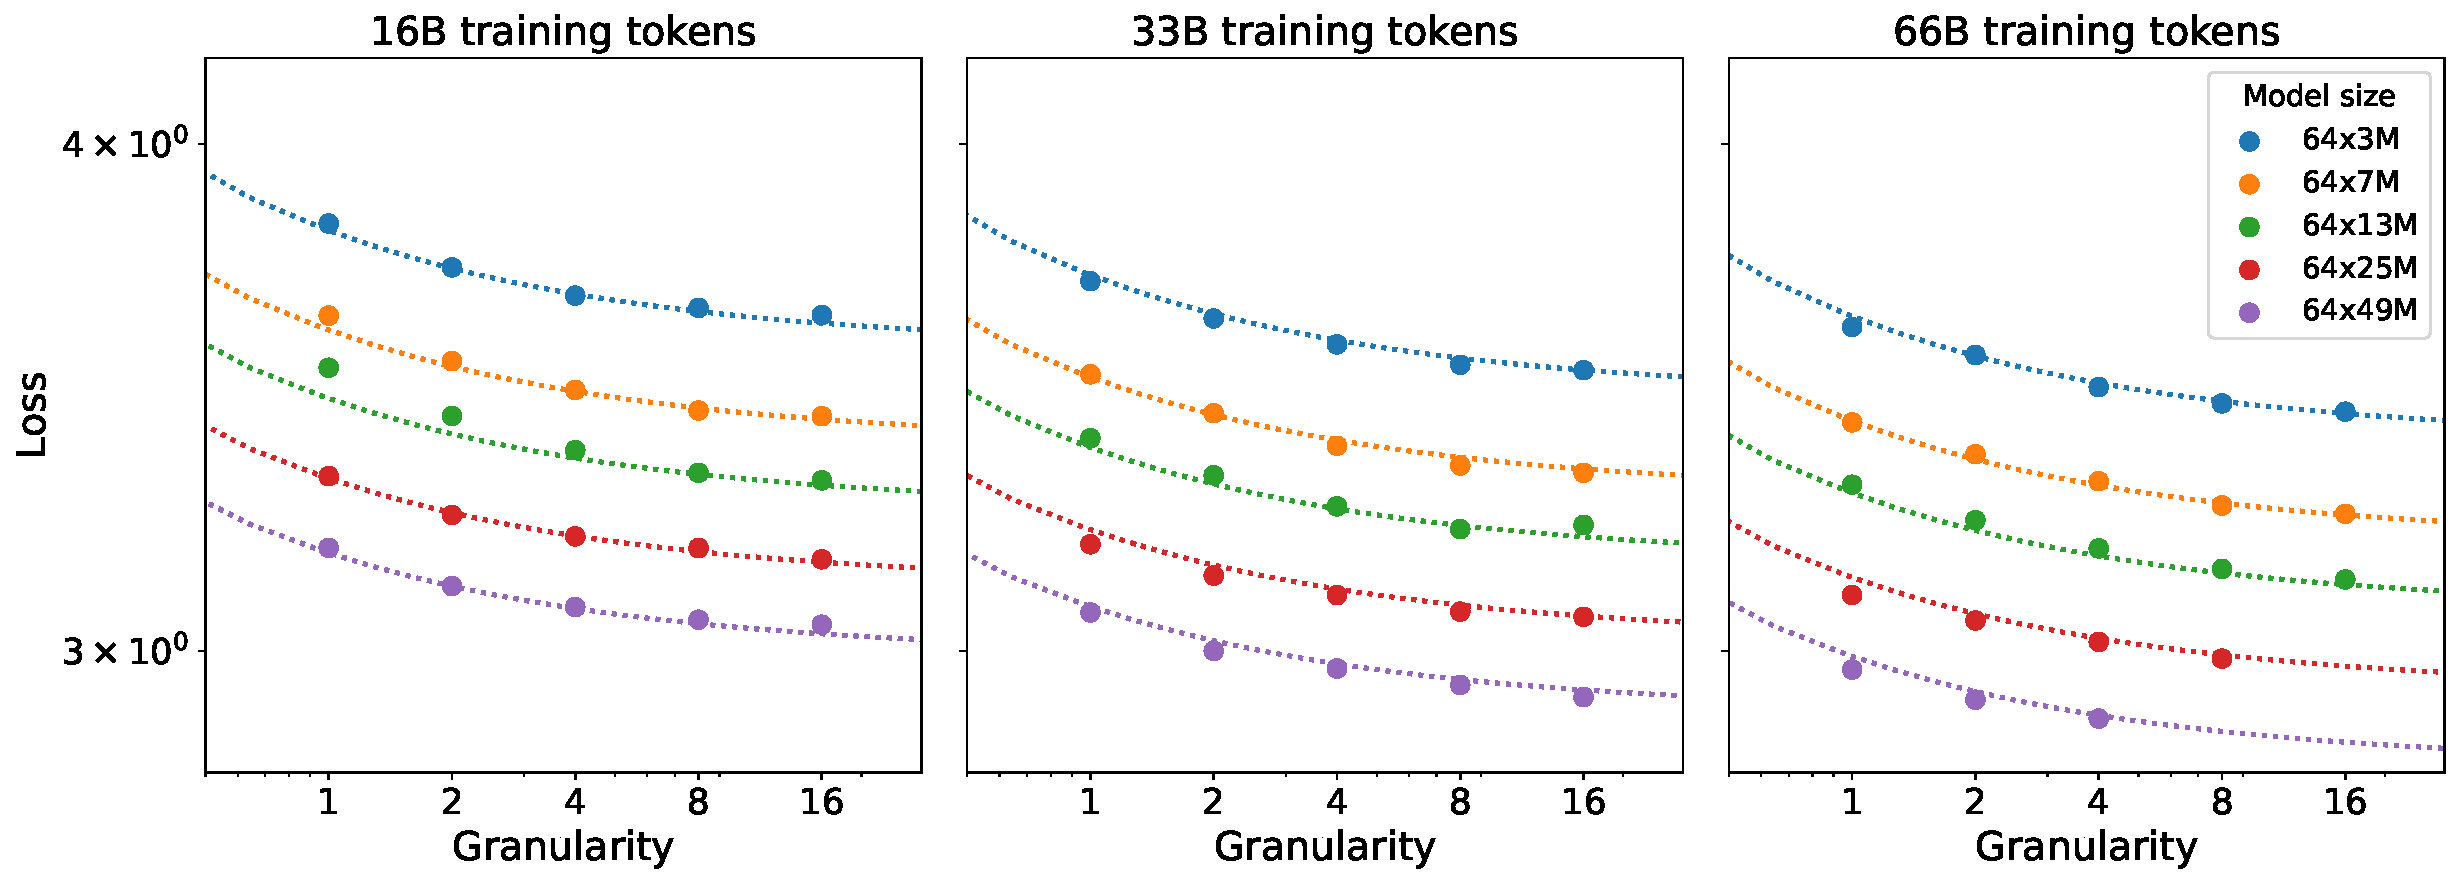
\includegraphics[width=.99\textwidth]{figures/final_fit_6.pdf}
  % \medskip
  \caption{Fit of the scaling laws compared to the experimental results.}
  \label{fig:scalinglaws}
\end{figure*}
Subsequently, we fit parameters in Eq. \ref{eq:loss_moe} to describe the scaling of MoE. For comparison, we also perform fitting for dense transformer given by Eq.~\ref{eq:chinchilla}. Similarly to \cite{hoffmann2022training}, we use Huber loss \citep{huber_loss}, with $\delta=0.1$. The optimization is performed using the BFGS algorithm. We include a weight decay of $5e-4$ to enhance generalization. We start with fitting parameters in Eq.~\ref{eq:loss_moe} and then find architecture-dependent coefficients $\alpha, \beta, A$ and $B$ in Eq.~\ref{eq:chinchilla}. We observe a good fit, with $\text{RMSE}=0.015$. The values are presented in Table \ref{tab:coeffs_scaling}. We depict the results in Figure~\ref{fig:scalinglaws}. 

\newpage
\subsection{Fitting the Parametric Scaling Law}\label{sub:parametric}
% \begin{align}\label{eq:loss_moe_num}
% \begin{split}
%     \mathcal{L}=
%     0.472 + \left(\frac{2.07}{G^{0.584}}+ 18.10\right)\frac{1}{N^{0.115}} + \frac{30.83}{D^{0.147}}.
% \end{split}
% \end{align}
\begingroup
\begin{table}[h]
    \centering
        \setlength{\tabcolsep}{5pt} 
    \caption{Values of the fitted coefficients.}
    \vspace{0.2cm}
    \begin{tabular}{ccccccccc}
        \toprule
        Model  & a & $\alpha$ & b & $\beta$ & g & $\gamma$ & c \\
        \midrule        
        MoE  & 18.1 & 0.115 & 30.8 & 0.147 & 2.1 & 0.58 & 0.47 \\ 
        Dense & 16.3 & 0.126 & 26.7 & 0.127 & - & - & 0.47\\
        \bottomrule
    \end{tabular}
    \label{tab:coeffs_scaling}
\end{table}
\endgroup

We validate the stability of the fit by excluding the top $20\%$ of models with the lowest perplexity and finding the coefficients based on the remaining experiments. We observe that the formula remains almost unchanged in this scenario (see Table \ref{tab:coeffs_valid} in Appendix \ref{app:coeffs_valid}). The validation RMSE is 0.019. Results are depicted in Figure~\ref{fig:valid_wall} (a).  

\begin{figure*}[t]
  \centering
  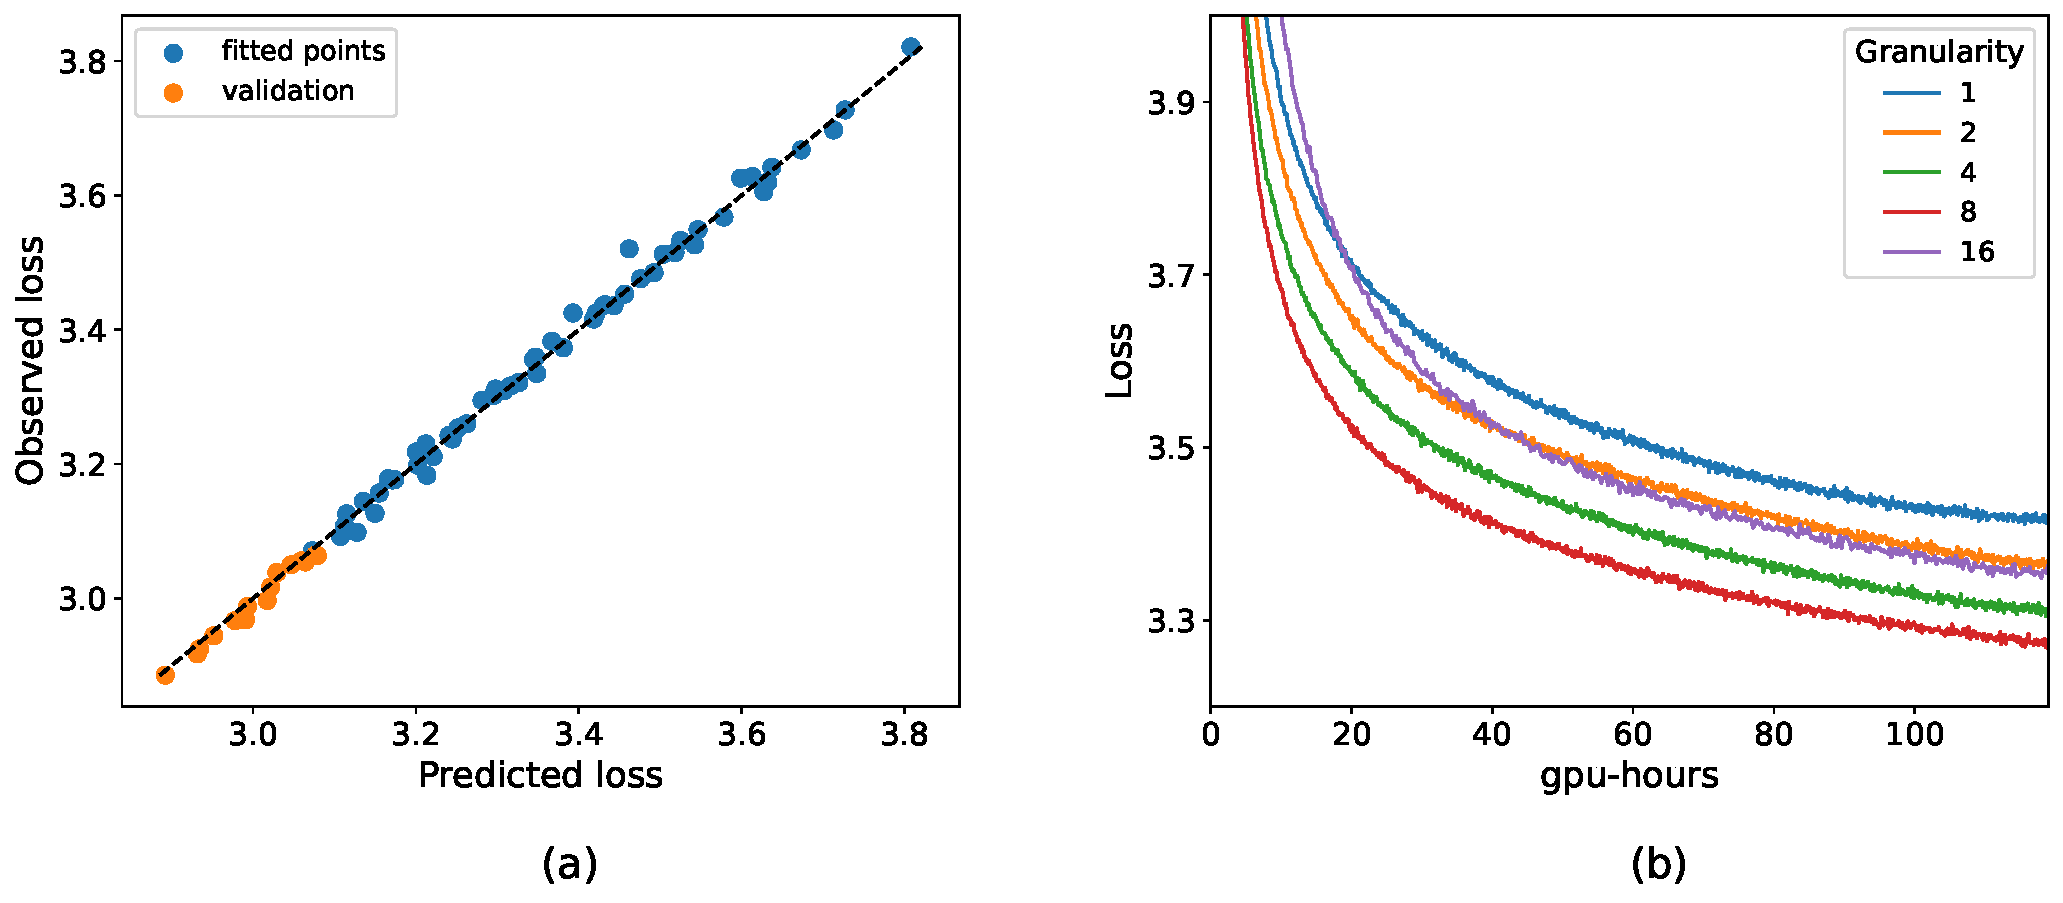
\includegraphics[width=.9\textwidth]{figures/valid_wall_clock.pdf}
  % \medskip
  \caption{\textbf{(a)} Validation of the scaling laws. \textbf{(b)} Training loss curves for model with $N=64 \times 7M$, $D=66B$ tokens, measured against wall-clock time on NVIDIA A100 GPU. $G=8$ leads to the best performance, as for $G=16$ the routing cost dominates gains from granularity. We model the increased cost of routing by measuring FLOPs for each configuration.}
  \label{fig:valid_wall}
\end{figure*}

% \begin{figure}[ht!] 
% \centering
% \includegraphics[width=0.45\textwidth]{icml2024/figures/validation.pdf}
% \caption{Validation of the fit.}
% \label{fig:validate}
% \end{figure}


\subsection{MoE Scaling Properties}\label{sub:scaling_properties}
%\ps{Ja nie rozumiem początku tego zdania.}
Comparing the part of the formula that approximates underfitting (that is, dependent on training tokens) in MoE ($30.8D^{-0.147}$) and Transformer ($26.7D^{-0.127}$), we can infer that MoE models need longer training to perform competitively but scale better after reaching that point. Nonetheless, this moment may still precede the compute optimal for both models.
%This is consistent with the common practice of longer training runs for sparse models present i.e in \cite{clark2022unified}. 
On the other hand, we can see that the exponent on dense models $\alpha=-0.126$ scales better with a total number of parameters than the MoE counterpart $\alpha=-0.115$. This should not be surprising since dense models use all parameters on each token contrary to MoE, which gains a computational advantage by activating only a subset of them. Therefore, the fair comparison of the performance has to take into account FLOPs used by each model type. In the next section, we find compute-optimal granularity for a given FLOP budget. 

% \jk{poprzednia wersja:}
% To fit this equation, similarly to \cite{hoffmann2022training}, we use BFGS algorithm working in log-scale. In order to compare our laws with baseline dense models, we also tune vanilla chinchilla scaling law within our training setup. However, for a fair comparison, both methods should have the same dataset bias $L_0$. Therefore we sweep over values from $(0,2)$ using intervals of $0.1$ and choose the value that gives us lowest approximation error for the fitted law, summed for both model classes. This also helps with the numerical stability of the approximation.
% Now we fit this equation and observe on figure \ref{fig:error} that this functional form allows for accurate prediction of the loss\jk{I would rather put the exact fitted values in the table} \sj{Maybe in the table as well, but I really like to see equation as a whole. Provides intuition, and it'll sell.}:

% \begin{align*}
%     L_f(N,D,G) = 0.5 + (5.52G^{-0.11}+{12.2})N^{-0.10} \\
%     + {485}D^{-0.28}
% \end{align*}
% \ps{tutaj brakuje jakiejś analizy błędów, np. 10 i 90 centyl}
% \subsection{Analysis of the Fitted Equation}\label{sub:analysis}
% \jk{Zakomentowałem część, która już jest w poprzednim fragmencie}
% % These parameters show, that granularity does not have interaction with training steps, however the interaction with number of parameters $N$ is significant and is the one responsive for the better performance of granular models. Therefore, we can reduce our scaling law to:
% % \begin{align*}
% %     L_s(N,D,G) = 0.5 + (2G^{-0.53}+{16.4})N^{-0.1} + 504D^{-0.28}
% % \end{align*}

% % \mk{to chyba jest do poprzedniego zdania, więc 'while'?} While the baseline fitted to $ 0.5 + 17.9N^{-0.14} + 30D^{-0.12}$. 
% Since in dense models, the tokens underfitting approximation is $30D^{-0.12}$, comparing to $504D^{-0.28}$ we can infer, that MoE models need longer training to perform competitively, but scale better after reaching that point. On the other hand, we can see that the exponent on dense models $N^{-0.14}$ scales better with number of parameters than the MoE counterpart $N^{-0.1}$. This should not be surprising, since dense models use all parameters on each token contrary to MoE, which  gain advantage by using computational power more efficiently. Therefore, final assessment of the performance has to take into account FLOPs used by each type of model.

% \jk{Na razie zakomentowuję quality of the fit. Ta informacja jest zawarta już na obrazku "Fit of the scaling law compared to experimental results". Dodatkowo myślę że damy osobny wykres "quality of the fit" z walidacją.}
% \begin{figure}[ht]
% \centering
% \includegraphics[width=0.4\textwidth]{icml2024/figures/error.png}
% \caption{Quality of the fit (MSE=0.0011). Similarity to \cite{hoffmann2022training}, error is higher on smaller models due to use of Huber loss, but prediction is not biased by granularity. \sj{Apart from the chart, it would be convincing to get some numbers - e.g. average bias/residual for each granularity; percent of variance unexplained by our scaling law, etc.} \janek{tutaj chyba lepszym argumentem, ze dziala i nie jest biased by granularity jest ten wykres \ref{fig:line}}}
% \label{fig:error}
% \end{figure}


%\begin{figure*}[ht]
%\centering
%\includegraphics[width=1.0\textwidth]{icml2024/figures/noline.png}
%\caption{A picture like that will be here. Caption: We verify our scaling results on the 3B scale. The model is }
%\label{fig:no_line}
%\end{figure*}

% \begin{figure*}[ht]
% \centering
% \includegraphics[width=0.7\textwidth]{icml2024/figures/intuition.png}
% \caption{(Left): Varying. (Right): ...}
% \label{fig:intuition}
% \end{figure*}

% \begin{figure*}[ht]
% \centering
% \includegraphics[width=1.0\textwidth]{icml2024/figures/gran_linear.png}
% \caption{Verification of our unified scaling laws for different training hyper-parameters. Granularity seem to not bias our loss predictions. \janek{tutaj musimy wstawic wykres faktycznej weryfikacji} }
% \label{fig:line}
% \end{figure*}

%\begin{figure}[ht]
%\centering
%\includegraphics[width=0.5\textwidth]{icml2024/figures/predict_scaling.png}
%\caption{A picture like that will be here. Caption: We verify our scaling results on the 3B scale. The model is }
%\label{fig:two_times}
%\end{figure}
